\icode{E-MI-SI-L3-261109-002}
如图所示，一个半球形的碗放在桌面上，碗口水平，\(O\)是球心，碗的内表面光滑。一根轻质杆的两端固定有两个小球，质量分别是\(m_1\)、\(m_2\)。当它们静止时，\(m_1\)、\(m_2\)与球心的连线跟水平面分别成\qty{60}{\degree}，\qty{30}{\degree}角，则碗对两小球的弹力大小之比是\paren[]

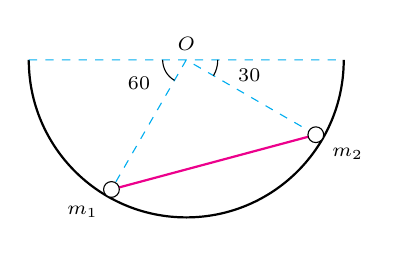
\begin{tikzpicture}[font=\scriptsize]
	\draw[thick] (2,0) arc(0:-180:2);
    \draw[thick,magenta] (-30:1.9)--(-120:1.9);
	\draw[dashed,cyan] (-120:2)node[below left,black]{\(m_1\)}--(0,0)--(-30:2)node[below right,black]{\(m_2\)} (-2,0)--(2,0);
	\draw[fill=white] (-30:1.9) circle(.1) (-120:1.9) circle(.1);
	\fill (0,0)node[above]{\(O\)};
	\draw (.4,0) arc(0:-30:.4) (-.3,0) arc(-180:-120:.3);
	\node at(-.6,-.3){\qty{60}{\degree}};
	\node at(.8,-.2){\qty{30}{\degree}};
\end{tikzpicture}
\begin{choices}
	\item\(1:2\)
	\item\(\sqrt{3}:1\)
	\item\(1:\sqrt{3}\)
	\item\(\sqrt{3}:2\)
\end{choices}
\begin{answer}
	B\qquad 提示：
\end{answer}